\documentclass[12pt,a4paper]{article}

% ===== LuaLaTeX: современные векторные шрифты =====
\usepackage{fontspec}           % для работы с TrueType/OpenType шрифтами
\setmainfont{Times New Roman}   % или Arial, Libertinus Serif, etc.

% ===== Языки и кодировка =====
\usepackage[english,russian]{babel}
\usepackage{csquotes}           % для кавычек

% ===== Математика =====
\usepackage{amsmath}
\usepackage{amsfonts}
\usepackage{amssymb}

% ===== Графика =====
\usepackage{graphicx}
\usepackage{tikz}
\usepackage{tkz-euclide}
\usepackage{pgfplots}
\pgfplotsset{compat=1.18} 

\usetikzlibrary{patterns}
\usepackage{float}
\usepackage{wrapfig}

% ===== Таблицы =====
\usepackage{multirow}
\usepackage{booktabs}
\usepackage{siunitx}
\usepackage{array}

% ===== Оформление =====
\usepackage[left=1cm,right=1cm,top=1cm,bottom=2cm]{geometry}
\usepackage{setspace}
\usepackage{indentfirst}
\usepackage{microtype}          % улучшает качество шрифтов
\usepackage{hyperref}

% ===== Вспомогательное =====
\usepackage{calc}
\usepackage{subfigure}

\usepackage{listings}
\usepackage{xcolor}

% Настройки для Python
\lstset{
	language=Python,
	basicstyle=\ttfamily\small,
	keywordstyle=\color{blue}\bfseries,
	stringstyle=\color{red},
	commentstyle=\color{green!50!black},
	numbers=left,
	numberstyle=\tiny\color{gray},
	stepnumber=1,
	numbersep=5pt,
	backgroundcolor=\color{gray!10},
	frame=single,
	breaklines=true,
	breakatwhitespace=true,
	tabsize=4,
	showspaces=false,
	showstringspaces=false,
	captionpos=b
}

\title{Быстрое умножение многочленов с помощью преобразования Фурье}
\author{Тодоров Николай}
\date{\today}

\begin{document}

\maketitle

\section{Дискретное преобразование Фурье}
Пусть дан периодический сигнал - $\{x_n\}_{n=0}^{N-1}$

Напомним, что прямое дискретное преобразование Фурье - DFT - описывается формулой:

\[X_k = \sum_{n = 0}^{N-1} x_n e^{-2\pi i k n / N} \text{;}\]
обратное дискретное преобразование Фурье - IDFT - в свою очередь описывается формулой:
\[x_n = \dfrac{1}{N} \sum_{k = 0}^{N-1} X_k e^{2\pi i k n / N}\]

Заметим, что DFT является линейным операторм, действующим в конечномерном пространстве.
Поэтому его можно представить в виде матрицы:

\[X_k = \sum_{n=0}^{N-1}M_{kn}x_n \text{, } M_{kn} = e^{-2\pi i k n /N} \] 

\section{Трактовка DFT через многочлены}

Как мы показали выше, DFT можно представить в виде матрицы.
Выпишем эту матрицу в явном виде

\[\mathcal{F} = 
\begin{bmatrix}
1 & 1 & 1 & 1 & \dots & 1 \\
1 & \omega_n & \omega_n^2 & \omega_n^3 & \dots & \omega_n^{n-1} \\
1 & \omega_n^2 & \omega_n^4 & \omega_n^6 & \dots & \omega_n^{2(n-1)} \\
1 & \omega_n^3 & \omega_n^6 & \omega_n^3 & \dots & \omega_n^{3n-1} \\
\vdots & \vdots & \vdots & \vdots & \ddots \\
1 & \omega_n^{n-1} & \omega_n^{2(n-1)} & \omega_n^{3(n-1)} & \dots & \omega_n^{(n-1)^2} \\
\end{bmatrix}
\]

$\mathcal{F}_{jk} = \omega_n^{(j-1)(k-1)} \text{, } 
\omega_n = e^{-2\pi i / n}
\text{, } j = 1 \text{, } \dots \text{, } n
\text{, } k = 1 \text{, } \dots \text{, } n$ 

Заметим, что это есть матрица Вандермонда, которая используется
в задаче интерполяции многочленами. Составим многочлен

\[p(x) = a_0 + a_1 x + \cdots + a_{n-1}x^{n-1} \]

Его значения в точках 

\[x_0 = 1 \text{, } x_1 = \omega_n \text{, } x_2 = \omega_n^2
\dots \text{, } x_{n-1} = \omega_n^{n-1}\]

дадут нам фурье-образ вектора $a = (a_0 \text{, } 
a_1 \text{, } \dots \text{, } a_{n-1} )$

Очевидно тогда, что если мы знаем значения многочлена в точках $x_k$, 
то мы можем, используя IDFT, найти коэффициенты этого многочлена

Теперь мы можем описать алгоритм быстрого перемножения многочленов.
Пусть нам даны многочлены:

\[p(x) = a_0 + a_1 x + \cdots + a_{n-1}x^{n-1} \]
\[q(x) = b_0 + b_1 x + \cdots + b_{m-1}x^{m-1} \]

Чтобы найти их произвдеение

\[(q \cdot p)(x) = c_0 + c_1 x + \cdots + c_{n+m-2}x^{n+m-2}\]

надо применить DFT к коэффициентам данных многочленов (таким образом мы получим
их значения в точках $x_k$), затем применить IDFT к вектору $C$:

\[C_k = q(x_k)p(x_k)\]

\section{Тестирование метода}

Измерим теперь скорость работы данного метода и сравним ее
с обычном методом перемножения многочленов. Алгоритм выше эффективнее простого перемножения коэффициентов,
если использовать FFT - быстрое преобразование Фурье.
FFT использует определенные симметрии комплексных экспонент, 
засчёт чего не приходится делать так много вычислительных операций. 

\begin{figure}[H]
	\centering
	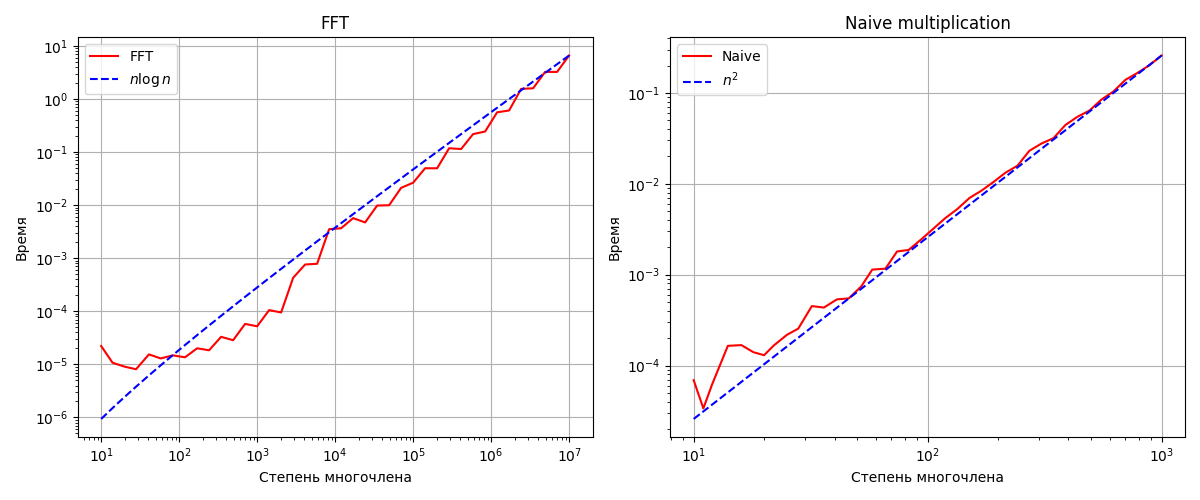
\includegraphics[width=1\textwidth]{Comparison.png}
	\caption{Сравнение двух методов}
\end{figure}
\end{document}